\documentclass[journal]{vgtc}                % final (journal style)

\usepackage{indentfirst} %MCW added

%% These few lines make a distinction between latex and pdflatex calls and they
%% bring in essential packages for graphics and font handling.
%% Note that due to the \DeclareGraphicsExtensions{} call it is no longer necessary
%% to provide the the path and extension of a graphics file:
%% 
\includegraphics{diamondrule} is completely sufficient.
%%
\ifpdf%                                % if we use pdflatex
  \pdfoutput=1\relax                   % create PDFs from pdfLaTeX
  \pdfcompresslevel=9                  % PDF Compression
  \pdfoptionpdfminorversion=7          % create PDF 1.7
  \ExecuteOptions{pdftex}
  \usepackage{graphicx}                % allow us to embed graphics files
  \DeclareGraphicsExtensions{.pdf,.png,.jpg,.jpeg} % for pdflatex we expect .pdf, .png, or .jpg files
\else%                                 % else we use pure latex
  \ExecuteOptions{dvips}
  \usepackage{graphicx}                % allow us to embed graphics files
  \DeclareGraphicsExtensions{.eps}     % for pure latex we expect eps files
\fi%

\usepackage{microtype}                 % use micro-typography (slightly more compact, better to read)
\PassOptionsToPackage{warn}{textcomp}  % to address font issues with \textrightarrow
\usepackage{textcomp}                  % use better special symbols
\usepackage{mathptmx}                  % use matching math font
\usepackage{times}                     % we use Times as the main font
\renewcommand*\ttdefault{txtt}         % a nicer typewriter font
\usepackage{cite}                      % needed to automatically sort the references

%% Paper title.
\title{Project Title Here \\
CS 725/825, Fall 2017}

%% This is how authors are specified in the journal style

%% indicate IEEE Member or Student Member in form indicated below
\author{FirstName1 LastName1 and FirstName2~LastName2\\
Department of Computer Science\\
Old Dominion University\\
Norfolk, VA 23529\\
\{username1, username2\}@cs.odu.edu
}
\authorfooter{
}

%other entries to be set up for journal
\shortauthortitle{Biv \MakeLowercase{\textit{et al.}}: Global Illumination for Fun and Profit}
%\shortauthortitle{Firstauthor \MakeLowercase{\textit{et al.}}: Paper Title}

%% Abstract section.
\abstract{Duis autem vel eum iriure dolor in hendrerit in vulputate
velit esse molestie consequat, vel illum dolore eu feugiat nulla
facilisis at vero eros et accumsan et iusto odio dignissim qui blandit
praesent luptatum zzril delenit augue duis dolore te feugait nulla
facilisi. Lorem ipsum dolor sit amet, consectetuer adipiscing elit,
sed diam nonummy nibh euismod tincidunt ut laoreet dolore magna
aliquam erat volutpat. Ut wisi enim ad minim veniam, quis nostrud exerci tation ullamcorper
suscipit lobortis nisl ut aliquip ex ea commodo consequat. Duis autem
vel eum iriure dolor in hendrerit in vulputate velit esse molestie
consequat, vel illum dolore eu feugiat nulla facilisis at vero eros et
accumsan et iusto odio dignissim qui blandit praesent luptatum zzril
delenit augue duis dolore te feugait nulla facilisi.%
} % end of abstract

%% Uncomment below to include a teaser figure.
\teaser{
  \centering
  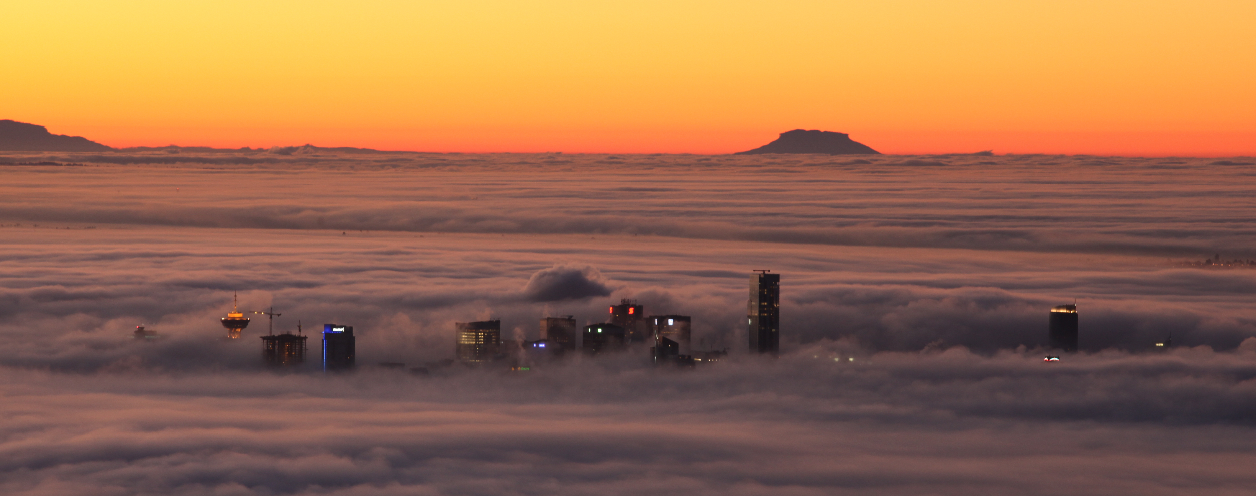
\includegraphics[width=\linewidth]{CypressView}
  \caption{In the Clouds: Vancouver from Cypress Mountain. Note that the teaser may not be wider than the abstract block.}
	\label{fig:teaser}
}

%% Uncomment below to disable the manuscript note
\renewcommand{\manuscriptnotetxt}{}

%% Copyright space is enabled by default as required by guidelines.
%% It is disabled by the 'review' option or via the following command:
 \nocopyrightspace

\vgtcinsertpkg

%%%%%%%%%%%%%%%%%%%%%%%%%%%%%%%%%%%%%%%%%%%%%%%%%%%%%%%%%%%%%%%%
%%%%%%%%%%%%%%%%%%%%%% START OF THE PAPER %%%%%%%%%%%%%%%%%%%%%%
%%%%%%%%%%%%%%%%%%%%%%%%%%%%%%%%%%%%%%%%%%%%%%%%%%%%%%%%%%%%%%%%%

\begin{document}

%% The ``\maketitle'' command must be the first command after the
%% ``\begin{document}'' command. It prepares and prints the title block.

%% the only exception to this rule is the \firstsection command
\firstsection{Introduction}

\maketitle

Provide an overview of the problem that you are addressing with your visualization

Discuss the questions that a user will be able to answer or explore with your visualization, including the abstract tasks

\section{Related Work}

Describe and cite any papers or other visualizations that have influenced your work.  Examples of citations \cite{alkwai-tois17}

\cite{berlin-jcdl17, alnoamany-websci17, weigle-capwic15}

\begin{figure}[tb]
 \centering % avoid the use of \begin{center}...\end{center} and use \centering instead (more compact)
 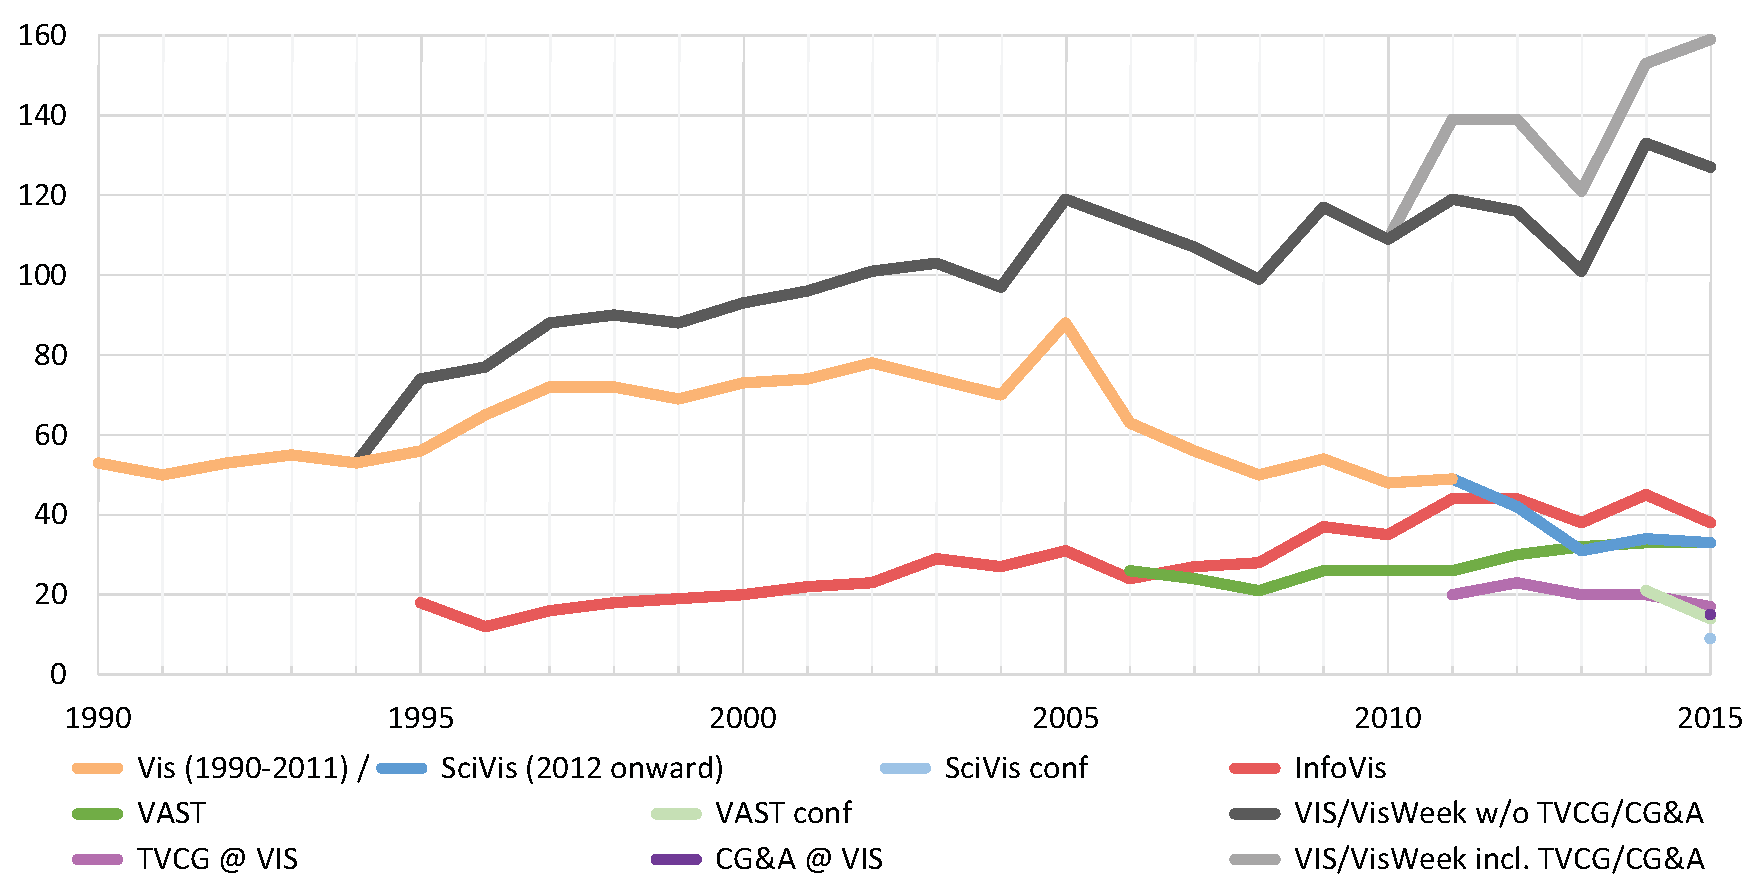
\includegraphics[width=\columnwidth]{paper-count-w-2015-new}
 \caption{A visualization of the 1990--2015 data. The image is from \cite{Isenberg:2017:VMC} and is in the public domain.}
 \label{fig:sample}
\end{figure}

\section {Data}
Describe the data used in your visualization, including citations and links to where it was obtained

\section{Visualization}
Describe the main features and idioms used in your visualization

\subsection{Design Decisions}
This may be a subsection of the Visualization section.

Discuss any design decisions made, including those made at the data/task abstraction level and the visual encoding/interaction idiom level (as done in Chapter 4).

\begin{figure*}
 \centering
 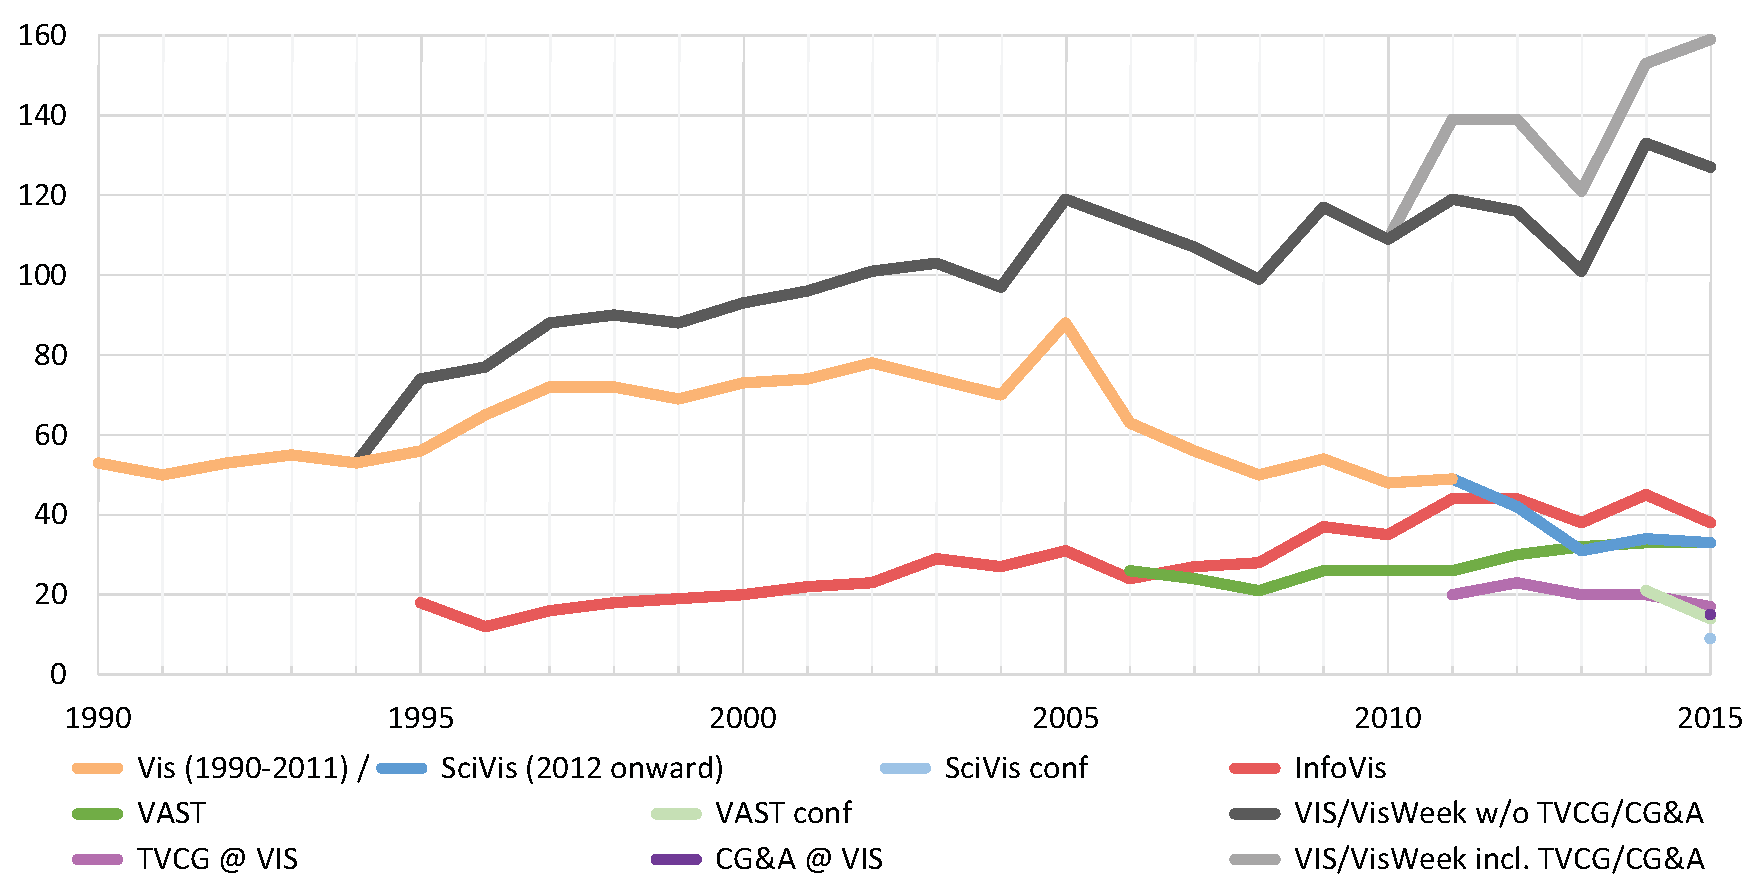
\includegraphics[width=0.8\linewidth]{paper-count-w-2015-new}
 \caption{Showing a single-column image over the two-column text.}
 \label{fig:sample-2}
\end{figure*}

\section{Analysis}

Analyze your system using the what/why/how framework, including creating a table as in Chapter 7. If you use multiple idioms, you may need to include multiple tables.

There are some nice examples of how to frame this in Chapter 15.  For each of the visualization tools in that chapter, there's a table that describes things like "what: data", "what: derived", "why: tasks", "how: encode".

\section{Insights or Case Study}
Show a concrete example of how the visualization addresses the abstract tasks proposed

\section{Conclusions}
Give a summary of the problem and how your visualization has addressed it.


\section*{Final Thoughts}
This is an unnumbered section.

Describe your experience working on the project. What were problems you faced? What things did you learn?


\bibliographystyle{abbrv-doi}
\bibliography{paper-template}
\end{document}

